\documentclass[11pt,a4paper]{article}
\usepackage[utf8]{inputenc}
%\usepackage[spanish,es-tabla]{babel}
\usepackage[english]{babel}
\usepackage{amsmath}
\usepackage{amsfonts}
\usepackage{amssymb}
\usepackage{graphicx}
\usepackage{subcaption}
\usepackage{fancyvrb}

\usepackage{titling}


\usepackage[colorlinks=true, 
            linkcolor = blue,
            urlcolor  = blue,
            citecolor = black,
            anchorcolor = blue]{hyperref}

\usepackage{siunitx}

\usepackage[margin=0.8in]{geometry}

\date{March 6, 2019}

\pretitle{%
  \begin{center}
  \LARGE
  
\includegraphics[width=6cm]{uc3m}\\[\bigskipamount]
}
\posttitle{\end{center}}

\begin{document}
	
	\title{\textbf{Lab. 2\\\LARGE{Channel Coding}}}
	\author{Ignacio Condés Menchén\\Luis Alberto Pacheco Lorenzo\\Advanced Techniques in Signal Processing and Communications}
	\maketitle
	
\section*{Convolutional Encoding}
The function \texttt{encoding} enters the sequence into the coding scheme given by the coding matrix \texttt{G}. It works for any generic matrix, but the implementation has been tested with $\mathbf{G}(D) = [D^2 + 1,\  D^2+D+1]$ (as it is stated in the practice).\\

Later, it is passed through a BSC (\textit{Binary Symmetric Channel}), with a given error probability affecting each bit on an independent way.\\


Hence, we can compare the \textit{Bit Error Rate} vs. the \textit{Signal-to-Noise Ratio}, as seen on \autoref{fig:ber}.



\begin{figure}[h]
	\centering
	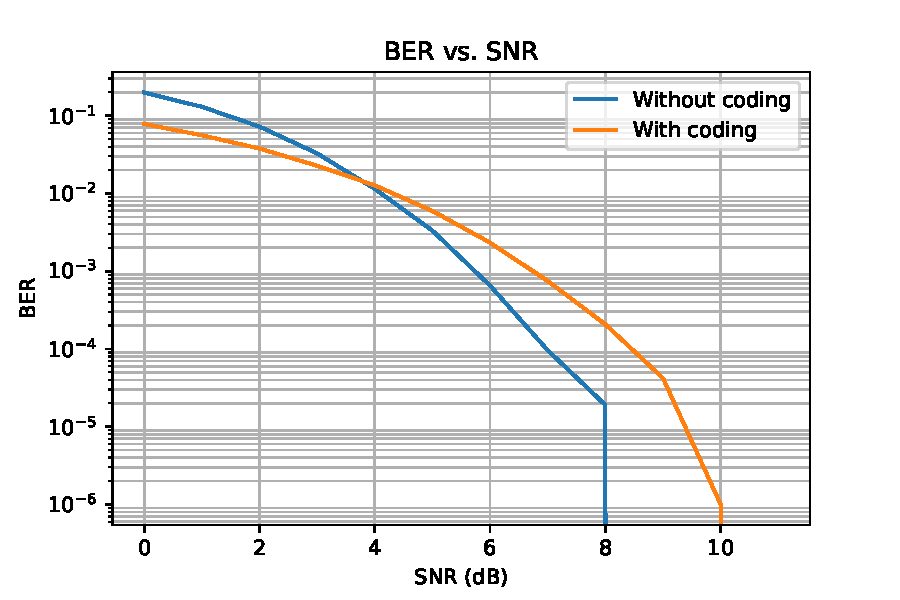
\includegraphics{figs/BER10000}
	\caption{BER vs SNR}
	\label{fig:ber}
\end{figure}



It can be seen that, on a higher SNR, a convolutional encoding is less worthy, as the bit error probability is too low for that. Hence, we can find an intersection point where both error probabilities are similar (approximately on a SNR value of 4 dB for this coding matrix \textbf{G}). Beyond that point, we can consider that the channel is good enough for a raw transmission without a protection redundancy.\\



\end{document}